\documentclass[a4paper, 11pt]{article}
\usepackage[slovene]{babel}
\usepackage[utf8]{inputenc}
\usepackage[T1]{fontenc}
\usepackage{amsfonts,amsmath,amssymb}
\usepackage{graphicx}
\usepackage{hyperref}
\usepackage{fancyvrb}


\newcommand{\R}{\mathbb R}
\newcommand{\N}{\mathbb N}
\newcommand{\Z}{\mathbb Z}
\newcommand{\C}{\mathbb C}
\newcommand{\Q}{\mathbb Q}

\begin{document}

\thispagestyle{empty}
\begin{center}
\begin{minipage}{0.75\linewidth}
    \centering
    {\Large Univerza v Ljubljani \\ Fakulteta za matematiko in fiziko}
    \\
    \vspace{7cm}

    {\uppercase{\LARGE \textbf{Bottleneck assignment in the plane}}} \\ Projekt pri predmetu Finančni praktikum \\
    \vspace{3cm}

    Avtorici:\\
    {\Large Lea Holc, Eva Rudolf\par}
    \vspace{7cm}

    {\Large Ljubljana, 2023}
\end{minipage}
\end{center}


\newpage
\tableofcontents
\newpage
\section{Navodilo}
Naj bosta $P$ in $Q$ dani množici točk v ravnini. Elementi množice $P$ predstavljajo proizvajalce 
(\textsl{providers}), elementi množice $Q$ pa porabnike (\textsl{clients}). Tako proizvajalci kot porabniki 
upravljajo z isto dobrino. Vsak proizvajalec $p \in P$ lahko proizvede $s_p > 0$ dobrine, za vsakega porabnika 
$q \in Q$ pa definiramo njegovo povpraševanje po dobrini kot $d_q > 0$. Predpostavimo, da je ponudba vseh 
prozvajalcev enaka povpraševanju vseh porabnikov. Cilj projekta je ugotoviti, ali za podano vrednost $\lambda$ 
proizvajalci lahko zadostijo potrebam porabnikov in sicer tako, da vsaka dobrina prepotuje pot največ $\lambda$. 

\section{Linearni program}
Ukvarjamo se s problemom maksimalnega pretoka, ki ga želimo predstaviti kot linearni program (LP).
Cilj je bil napisati linearni program, ki minimizira največjo razdaljo, ki jo mora prepotovati dobrina 
od proizvajalca do porabnika, pri čemer moramo zadostiti vsem potrebam, ki jih imajo porabniki, ne da 
bi presegli kapacitete, ki jih lahko proizvede posamezen proizvajalec. 
\subsection{Oznake}
Najprej uvedemo oznake. Naj bo $p_i$ za $i=1,\dots,m$ posamezen proizvajalec s koordinatami $(x_i,y_i)$ in 
$s_i$ za $i=1,2,\dots,m$ njegova proizvodnja dobrine. 
Naprej naj bo $q_j$ za $j=1,2,\dots,n$ posamezen porabnik s koordinatami $(w_j,z_j)$ in $d_j$ 
za $j=1,2,\dots,n$ njegovo povpraševanje 
po dobrini. Spomnimo se, da tako proizvajalci kot porabniki upravljajo z isto dobrino in predpostavimo, da velja
$$
\sum_{i=1}^m s_i = \sum_{j=1}^n d_j.
$$ 
S $c_{ij}$ označimo količino, ki jo proizvajalec $i$ dobavi porabniku $j$. Ker vsi proizvajlci ne 
dobavljajo vsem porabnikom, uvedemo še indikatorsko spremenljivko $b_{ij}$.
$$
b_{ij} = 
\begin{cases}
    0;\qquad \textrm{i-ti proizvajalec ne oskrbuje j-tega ponudnika} \\
    1;\qquad \textrm{i-ti proizvajalec oskrbuje j-tega ponudnika} \\
\end{cases} 
$$
Z $\lambda$ označimo maksimalno razdaljo, ki jo lahko prepotuje posamezna dobrina. To razdaljo 
želimo minimizirati.
\subsection{Pogoji}
Zapišimo še pogoje, s katerimi zadostimo potrebam posameznega porabnika in zmožnostim posameznega 
proizvajalca:
$$
\sum_{j=1}^n c_{ij} = s_i \text{ za } \forall i = 1,\dots,m 
$$
$$
\sum_{i=1}^m c_{ij} = d_j \text{ za } \forall j = 1,\dots,n 
$$
Za indikatorsko spremenljivko $b_{ij}$ lahko zapišemo $$0 \leq b_{ij} \leq 1 \text{ in } b \in \Z.$$
Veljati mora tudi $b_{ij}=0 \Rightarrow c_{ij}=0$, kar lahko zapišemo kot 
$$0 \leq c_{ij} \leq c_{ij}\cdot b_{ij}.$$
Omejimo še $\lambda$:
$$b_{ij}\cdot \sqrt{(x_i - w_j)^2+(y_i - z_j)^2} \leq \lambda.$$
\noindent
Naš cilj bo poiskati
$$
\min \max_{i,j} \sqrt{(x_j-x_i)^2 + (y_j-y_i)^2} \cdot c_{ij}.
$$

\section{Reševanje problema}
\subsection{Programiranje rešitev}
Glede na to, da se ukvarjamo z linearnim programiranjem, sva za zapis algoritmov 
uporabili programski jezik \emph{SageMath} v okolju \emph{CoCalc}. Napisali sva funkcije 
za generiranje točk, linearni program in dodatne funkcije za določitev pričakovane vrednosti $\lambda$
in za analizo časovne zahtevnosti. \par
Najprej sva definirali tri različne funkcije za generiranje množic točk proizvajalcev $P$ in 
porabnikov $Q$. To so funkcije \emph{kvadrat}, \emph{krog} in \emph{strani}, ki se -- kot
nam povedo njihova imena -- razlikujejo glede na to, v katerem območju generirajo točke.
Vsaka funkcija sprejme moč množice $P$, moč množice $Q$ in velikost območja (npr. polmer kroga pri
funkciji \emph{krog}). \par
Vsaka izmed teh funkcij za vsakega proizvajalca oz. točko iz $P$ določi, koliko proizvede,
ter za vsakega porabnika oz. točko iz $Q$, koliko porabi. \par
Naslednja funkicija, ki sva jo napisali, je funkcija \emph{program}, ki sprejme množici 
točk, ki jih vrnejo funkcije za generiranje točk. Ta funkcija deluje kot linearen program,
ki minimizira največjo razdaljo, ki jo mora prepotovati dobrina 
od proizvajalca do porabnika, pri čemer moramo zadostiti vsem pogojem, ki smo jih navedli v točki 2.2.
Vrne vrednost $\lambda$ (v programski kodi je to spremenjivka $z$), množico povezav in uteži povezav; torej
kolikšna količina dobrine potuje od proizvajalca $i$ do porabnika $j$. \par


\pagebreak
Programska koda za funkcijo \emph{program}:

\begin{verbatim}
    def program(s,d):
    m = len(s)
    n = len(d)
    p = MixedIntegerLinearProgram(maximization=False)
    b = p.new_variable(binary=True)
    c = p.new_variable(nonnegative=True)
    p.set_objective(p['l'])
    p.add_constraint((p['l']) >= 0)
    for i, ((sx, sy), sk) in enumerate(s):
        for j, ((dx, dy), dk) in enumerate(d):
            p.add_constraint(b[i, j] * sqrt((dx-sx)^2 + (dy-sy)^2) <= p['l'])
            p.add_constraint(c[i, j] >= 0)
            p.add_constraint(c[i, j] <= sk * b[i, j])
    for i, (sxy, sk) in enumerate(s):
        p.add_constraint(p.sum(c[i, j] for j in range(n)) == sk)
    for j, (dxy, dk) in enumerate(d):
        p.add_constraint(p.sum(c[i, j] for i in range(m)) == dk)
    z = p.solve()
    povezave = p.get_values(b)
    kolicine = p.get_values(c)
    return z, povezave, kolicine
\end{verbatim}

\subsection{Grafični prikaz rezultatov}
Na spodnjih grafih so prikazane rešitve za različne parametre in različne načine 
generiranja točk. Na grafih z manj točkami so prikazane tudi uteži povezav.
Le-ti sta na vsaki povezavi dve -- zgornja pomeni količino, ki jo proizvajalec $p_i$ dostavi
porabniku $q_i$, spodnja pa je razdalja med vozliščema.
Na grafih z več točkami so zaradi preglednosti uteži povezav izpuščene. \par
\pagebreak
Če za generiranje točk uporabimo funkcijo \emph{kvadrat}, dobimo naslednja dva grafa:
\begin{figure}[h!]
    \centering
    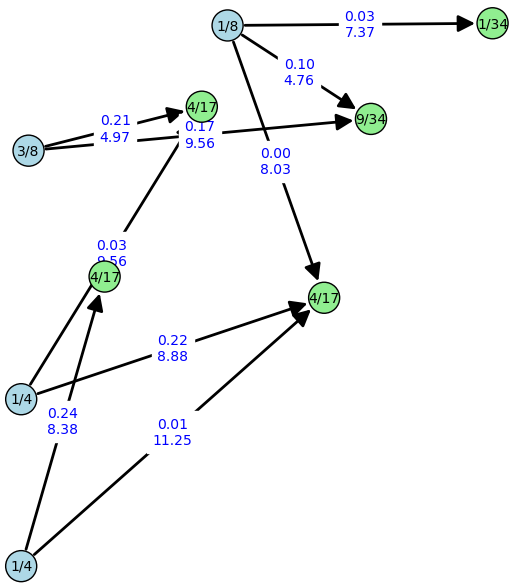
\includegraphics[scale=0.56]{kvadrat.png}
    \caption{Generiranje točk v kvadratu s stranico 20 za $|P|=4$, $|Q|=5$}
\end{figure}

\begin{figure}[h!]
    \centering
    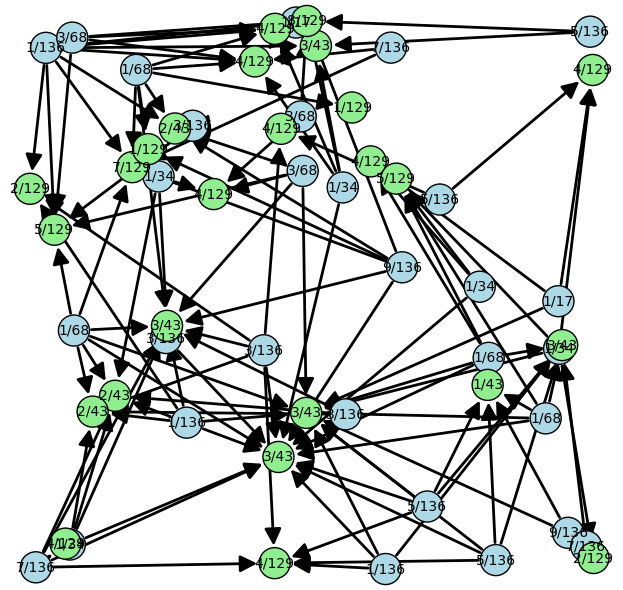
\includegraphics[scale=0.56]{kvadrat2.png}
    \caption{Generiranje točk v kvadratu s stranico 40 za $|P|=30$, $|Q|=25$}
\end{figure}
\noindent

Če uporabimo funkcijo \emph{krog}:
\begin{figure}[h!]
    \centering
    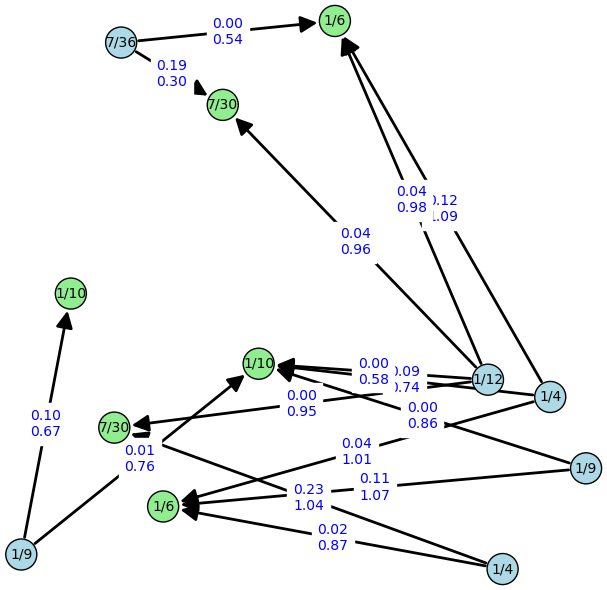
\includegraphics[scale=0.56]{krog.png}
    \caption{Generiranje točk v krogu s polmerom 1 za $|P|=6$, $|Q|=6$}
\end{figure}

\begin{figure}[h!]
    \centering
    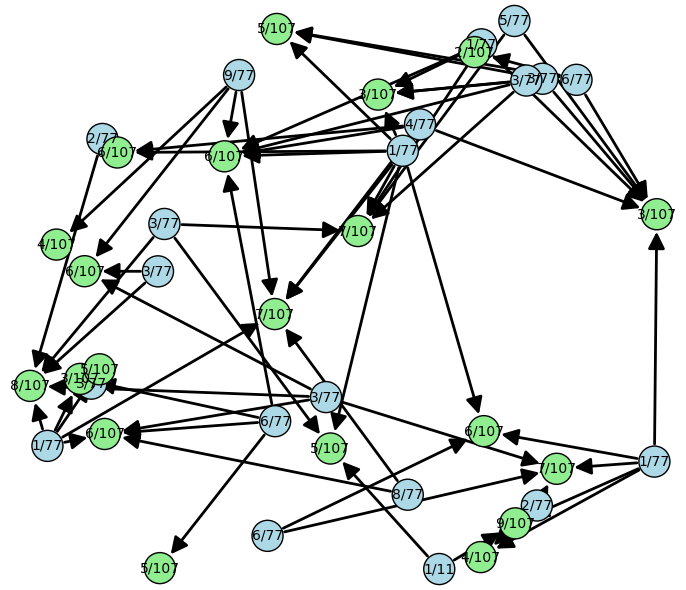
\includegraphics[scale=0.56]{krog2.png}
    \caption{Generiranje točk v krogu s polmerom 3 za $|P|=20$, $|Q|=20$}
\end{figure}
\pagebreak
\noindent
Za konec generiramo še točke na dveh vzporednih daljicah s pomočjo funkcije \emph{stani}:
\begin{figure}[h!]
    \centering
    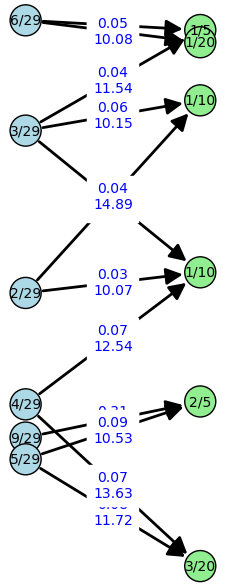
\includegraphics[scale=0.56]{stran.png}
    \caption{Generiranje točk na vzporednih daljicah za $|P|=6$, $|Q|=6$}
\end{figure}

\begin{figure}[h!]
    \centering
    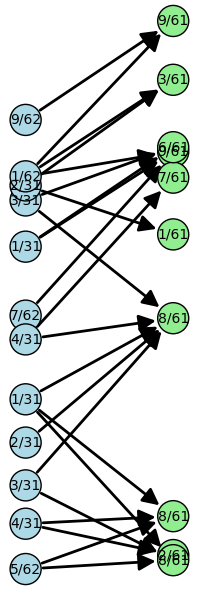
\includegraphics[scale=0.56]{stran2.png}
    \caption{Generiranje točk na vzporednih daljicah za $|P|=12$, $|Q|=10$}
\end{figure}

\pagebreak
\section{Analiza}
Da bi analizirali pričakovano vrednost razdalje $\lambda$, sva večkrat 
zagnali funkcijo \emph{program} s pomočjo funkcije \emph{simulacija}. Rezultate sva shranili
v \texttt{.csv} datoteko in s pomočjo programa \texttt{R} izrisali še histograme, ki kažejo
pričakovane vrednosti $\lambda$ za izbrane parametre v odvisnosti od tega, kje generiramo točke,
ki predstavljajo proizvajalce in porabnike. Rezultati so prikazani na spodnjih grafih.

\begin{figure}[h!]
    \centering
    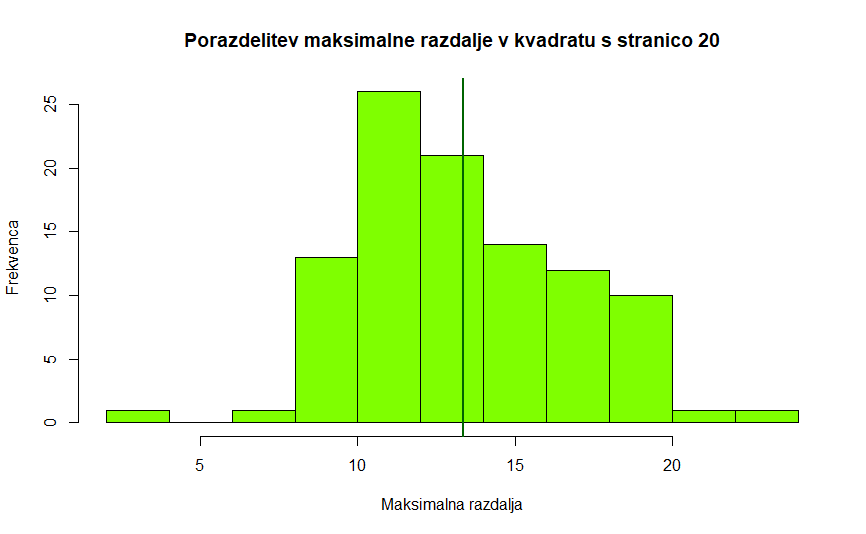
\includegraphics[scale=0.5]{porazdelitev_v_kvadratu.png}
\end{figure}

\begin{figure}[h!]
    \centering
    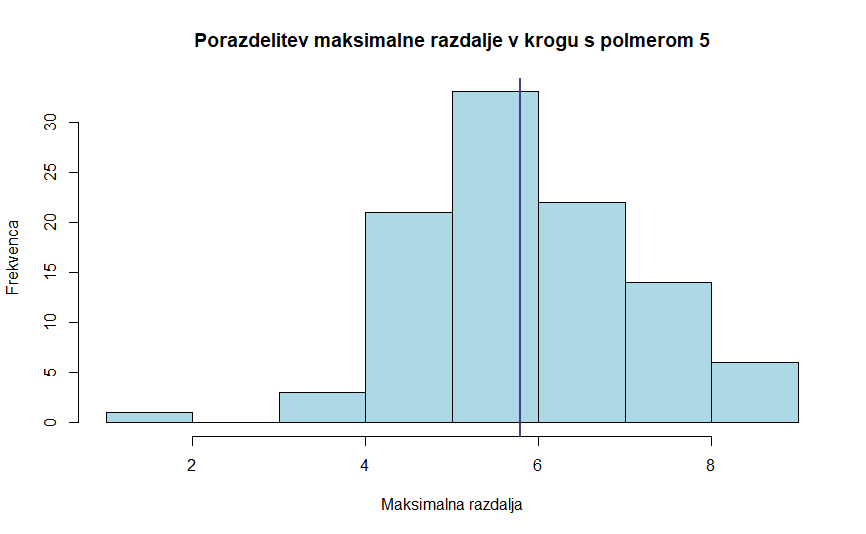
\includegraphics[scale=0.5]{porazdelitev_v_krogu.png}
\end{figure}

\clearpage
\begin{figure}[t!]
    \centering
    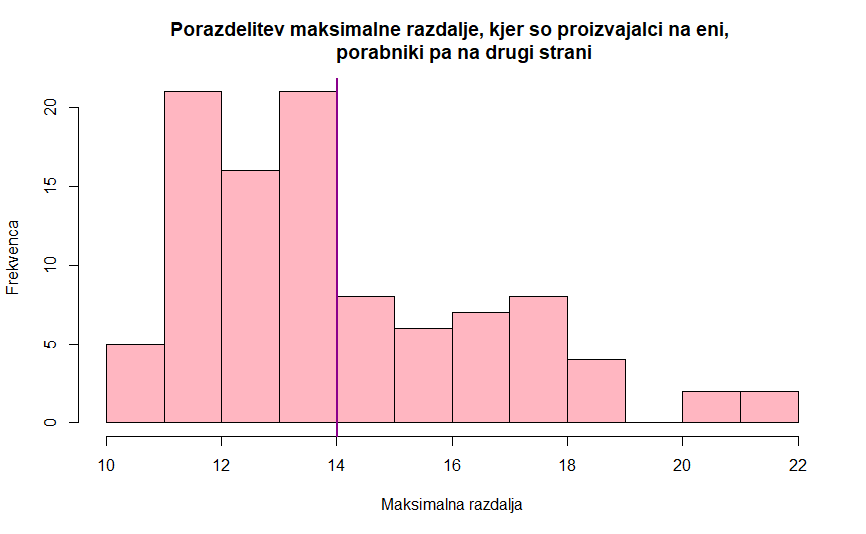
\includegraphics[scale=0.5]{porazdelitev_strani.png}
\end{figure}
\mbox{}


\end{document}